
%%%%%%%%%%%%%%%%%%%%%%% file typeinst.tex %%%%%%%%%%%%%%%%%%%%%%%%%
%
% This is the LaTeX source for the instructions to authors using
% the LaTeX document class 'llncs.cls' for contributions to
% the Lecture Notes in Computer Sciences series.
% http://www.springer.com/lncs       Springer Heidelberg 2006/05/04
%
% It may be used as a template for your own input - copy it
% to a new file with a new name and use it as the basis
% for your article.
%
% NB: the document class 'llncs' has its own and detailed documentation, see
% ftp://ftp.springer.de/data/pubftp/pub/tex/latex/llncs/latex2e/llncsdoc.pdf
%
%%%%%%%%%%%%%%%%%%%%%%%%%%%%%%%%%%%%%%%%%%%%%%%%%%%%%%%%%%%%%%%%%%%


\documentclass[runningheads,a4paper]{llncs}

\usepackage[cmex10]{amsmath}
\usepackage{amssymb}
\setcounter{tocdepth}{3}
\usepackage{graphicx}

\usepackage{url}
\urldef{\mailsa}\path|{peleska,huang}@uni-bremen.de|   

\urldef{\mailsb}\path|ana.cavalcanti@york.ac.uk|
\urldef{\mailsc}\path|adenilso@icmc.usp.br|


\newcommand{\keywords}[1]{\par\addvspace\baselineskip
\noindent\keywordname\enspace\ignorespaces#1}

\usepackage{float}
\usepackage{lscape}
\usepackage{lscape}

\usepackage{zed-csp}


\DeclareMathSymbol{\B}{\mathalpha}{AMSb}{"42}
\DeclareMathSymbol{\I}{\mathalpha}{AMSb}{"49}
\DeclareMathSymbol{\N}{\mathalpha}{AMSb}{"4E}
\DeclareMathSymbol{\Pwr}{\mathalpha}{AMSb}{"50}
\DeclareMathSymbol{\Q}{\mathalpha}{AMSb}{"51}
\DeclareMathSymbol{\R}{\mathalpha}{AMSb}{"52}
\DeclareMathSymbol{\Z}{\mathalpha}{AMSb}{"5A}
\DeclareMathSymbol{\Sol}{\mathalpha}{AMSb}{"53}

\newcommand{\obsv}[1]{{\cal O}(#1)}
\newcommand{\ctrl}[1]{{\cal C}(#1)}
\newcommand{\vdot}[1]{\stackrel{.}{#1}}
%\newcommand{\power}{\mathbf{P}}

\newcommand{\HS}{{\mathcal H}}

\newcommand{\Interval}{\I}

\newcommand{\ist}{\mbox{{\tt true}}}
\newcommand{\isf}{\mbox{{\tt false}}}
\newcommand{\emptytrace}{\langle~\rangle}
\newcommand{\abegin}{\mathbf{begin}}
\newcommand{\aend}{\mathbf{end}}
\newcommand{\alet}{\mathbf{let}}
\newcommand{\aendlet}{\mathbf{endlet}}
\newcommand{\ain}{\mathbf{in}}
\newcommand{\afor}{\mathbf{for}}
\newcommand{\adownto}{\mathbf{downto}}
\newcommand{\aforall}{\mathbf{foreach}}
\newcommand{\awhile}{\mathbf{while}}
\newcommand{\ado}{\mathbf{do}}
\newcommand{\aod}{\mathbf{od}}
\newcommand{\aenddo}{\mathbf{enddo}}
\newcommand{\aif}{\mathbf{if}}
\newcommand{\afi}{\mathbf{fi}}
\newcommand{\athen}{\mathbf{then}}
\newcommand{\aelse}{\mathbf{else}}
\newcommand{\aelseif}{\mathbf{elseif}}
\newcommand{\aendif}{\mathbf{endif}}
\newcommand{\ainout}{\mathbf{inout}}
\newcommand{\awhere}{\mathbf{where}}
\newcommand{\areturn}{\mathbf{return}}
\newcommand{\aout}{\mathbf{out}}
\newcommand{\aprocedure}{\mathbf{procedure}}
\newcommand{\afunction}{\mathbf{function}}
\newcommand{\abreak}{\mathbf{break}}
\newcommand{\Sup}[1]{\overline{#1}}
\newcommand{\Inf}[1]{\underline{#1}}


\newcommand{\taba}{\hspace*{3mm}}
\newcommand{\tabb}{\hspace*{6mm}}
\newcommand{\tabc}{\hspace*{9mm}}
\newcommand{\tabd}{\hspace*{12mm}}
\newcommand{\tabe}{\hspace*{15mm}}
\newcommand{\tabf}{\hspace*{18mm}}

\newcommand{\gca}[1]{{{#1}^{\vartriangleright}}}
\newcommand{\gcb}[1]{{{#1}^{\vartriangleleft}}}
\newcommand{\gclr}{{{\vartriangleleft\atop\longleftarrow}\atop
                   {\longrightarrow\atop\vartriangleright}}}



\newcommand{\Nat}{{\mathbb N}}
\newcommand{\Real}{{\mathbb R}}

\newcommand{\trans}{\longrightarrow}
\newcommand{\transxxx}[1]{\stackrel{#1}{\longrightarrow}}

\newcommand{\transp}{\longrightarrow_{\power}}
\newcommand{\transl}{\longrightarrow_{L}}
\newcommand{\transg}{\longrightarrow_{G}}
\newcommand{\transcfg}[1]{\stackrel{#1}{\longrightarrow}_{CFG}}
\newcommand{\isdefd}{=_{\mbox{\footnotesize def}}}
\newcommand{\equivdef}{\equiv_{\mbox{\footnotesize def}}}
\newcommand{\mitem}{\mbox{\em M-Item}}
%\newcommand{\fun}{\rightarrow}
%\newcommand{\pfun}{\not\rightarrow}
\newcommand{\currt}{\hat{t}}

%\newcommand{\dom}{\mbox{dom}}
%\newcommand{\ran}{\text{ran}}

\newcommand{\sigmaa}{\sigma_A}
\newcommand{\strictimplies}{\stackrel{\bullet}{\Rightarrow}}

\newcommand{\trl}{/\!/}


\newcommand{\q}{\textbf{q}}


\newcommand{\eqc}[2]{[#1;#2]}


\newcommand{\vest}{V_{\text{\sl est}}}
\newcommand{\vmax}{V_{\text{\sl MRSP}}}
\newcommand{\wout}{\mathsf{W}}
\newcommand{\eout}{\mathsf{EB}}
\newcommand{\areb}{\mathsf{allowRevokeEB}}
\newcommand{\sbia}{\mathsf{SBAvailable}}
\newcommand{\sbz}{\mathsf{sb}_0}
\newcommand{\ticmd}{\mathsf{TICmd}}
\newcommand{\dmicmd}{\mathsf{DMICmd}}

\newcommand{\sob}{\mathsf{speedOnBoard}}
\newcommand{\std}{\mathsf{speedToDriver}}
\newcommand{\pstd}{\mathsf{permittedSpeedToDriver}}
\newcommand{\csmsw}{\mathsf{csmSwitch}}
\newcommand{\sbicmd}{\mathsf{sbiCmd}}
\newcommand{\sbidisplay}{\mathsf{DMIdisplaySBI}}


\newcommand{\dvw}{\mathsf{dV}_{\mathsf{warning}}}
\newcommand{\dvs}{\mathsf{dV}_{\mathsf{sbi}}}
\newcommand{\dve}{\mathsf{dV}_{\mathsf{ebi}}}

 
\newcommand{\calcw}{\mathsf{dV\_warning(float)}}
\newcommand{\calcs}{\mathsf{dV\_sbi(float)}}
\newcommand{\calce}{\mathsf{dV\_ebi(float)}}
\newcommand{\calcstd}{\mathsf{calc\_speed\_to\_driver()}}
\newcommand{\calcpstd}{\mathsf{calc\_permitted\_speed\_to\_driver()}}
\newcommand{\calcsob}{\mathsf{calc\_speed\_onboard()}}

\newcommand{\trc}{\text{traces}}
\newcommand{\qtrc}{\text{qtraces}}
\newcommand{\iotrc}{\text{L}}


%\newtheorem{definition}{Definition}
%\newtheorem{property}{Property}
%\newtheorem{lemma}{Lemma}
%\newtheorem{theorem}{Theorem}
%\newtheorem{corollary}{Corollary}
%\newtheorem{property}{Property}

%\newtheorem{note}{Note}[section]



        
\newcommand{\xbox}{\unskip\nobreak\hfil\penalty50
      \hskip2em\hbox{}\nobreak\hfil$\Box$%
      \parfillskip=0pt\finalhyphendemerits=0 \par%
      
      \medskip
      \parfillskip=0pt plus 1fil
}
      
\newcommand{\dontshow}[1]{}    
\newcommand{\annot}[1]{\textbf{\textcolor{red}{#1}}}  




\newcommand{\ta}{\mathbf{A}}
\newcommand{\te}{\mathbf{E}}
\newcommand{\tx}{\mathbf{X}}
\newcommand{\tf}{\mathbf{F}}
\newcommand{\tg}{\mathbf{G}}
\newcommand{\tu}{\mathbf{U}}
\newcommand{\tr}{\mathbf{R}}
\newcommand{\tw}{\mathbf{W}}

\newcommand{\ttu}[1]{\mathbf{U}^{#1}}
\newcommand{\ttg}[1]{\mathbf{G}^{#1}}
\newcommand{\ttf}[1]{\mathbf{F}^{#1}}




\newcommand{\fsm}{\text{FSM}}
\newcommand{\dfsm}{\text{DFSM}}
\newcommand{\nfsm}{\text{NFSM}}
\newcommand{\refmod}{\mathit{Ref}}



 \newcommand{\passeq}{\underline{\text{pass}}_\sim}
\newcommand{\tfaileq}{\underline{\text{fail}}_\sim}

\newcommand{\passred}{\underline{\text{pass}}_\preceq}
\newcommand{\tfailred}{\underline{\text{fail}}_\preceq}



\newcommand{\pass}{\underline{\text{pass}}}
 \newcommand{\tfail}{\underline{\text{fail}}}
 
\newcommand{\xpass}[1]{{#1}_\text{pass}}
\newcommand{\xfail}[1]{{#1}_\text{fail}}

\newcommand{\tc}{{\text{TC}}}
\newcommand{\TS}{{\text{TS}}}
\newcommand{\DL}{{\text{DL}}}
\newcommand{\deadlock}{{\it deadlock}}
\newcommand{\DF}{\text{DF}}

\newcommand{\ii}[1]{\underline{#1}}
\newcommand{\inc}{\,{\rm I}\,}


\newcommand{\scov}{\text{SCOV}}
\newcommand{\after}{\text{-after-}}
\newcommand{\reduction}{\preceq}


\newcommand{\ps}{\le_s}
\newcommand{\pss}[1]{\stackrel{#1}{\ps}}


\newcommand{\pe}{\sim_s}
\newcommand{\pes}[1]{\stackrel{#1}{\pe}}
\newcommand{\ol}{\overline}
\newcommand{\diag}{\mathbf{diag}}
\newcommand{\primem}{\mathbf{prime}}


% ===========================================================================
\begin{document}

\mainmatter  % start of an individual contribution

% first the title is needed
\title{Finite Complete Suites for CSP Refinement Testing}

% a short form should be given in case it is too long for the running head
\titlerunning{CSP Refinement Testing}

% the name(s) of the author(s) follow(s) next
%
% NB: Chinese authors should write their first names(s) in front of
% their surnames. This ensures that the names appear correctly in
% the running heads and the author index.
%
\author{
Ana Cavalcanti\inst{1}
\and
Wen-ling Huang\inst{2}
\and
Jan Peleska\inst{2}
\and
Adenilso Simao\inst{3}
}
%
\authorrunning{Ana Cavalcanti, Wen-ling Huang, Jan Peleska, and Adenilso Simao}


\institute{
University of York, United Kingdom\\
\mailsb
\and
University of Bremen, Germany\\
\mailsa
\and
University of S{\~a}o Paulo, Brazil\\
\mailsc}

 
\maketitle 


\begin{abstract}




\keywords{Model-based testing, Complete testing theories, CSP, Refinement}
\end{abstract}

% =========================================================================

\section{Introduction}
\label{sec:intro}

% =================================================================================

\subsubsection*{Motivation}

Model-based testing (MBT) is an  active research field that is currently
integrated into industrial verification processes by many companies. This
holds particularly for the embedded and cyber-physical systems domain. While
MBT is applied in different flavours, we consider the most effective variant
to be the one where test cases and concrete test data, as well as checkers
for the expected results~(\emph{test oracles}), are automatically generated
from a reference model:~it guarantees the maximal return of investment for
the time and effort invested into creating the test model. The test suites
generated in this way, however, usually have different test strength,
depending on the generation algorithms applied.

For the safety-critical domain, test suites with guaranteed fault coverage
are of particular interest. For black-box testing, guarantees can be given
only if certain hypotheses are satisfied. These hypotheses are usually
specified by a \emph{fault domain}:~a set of models that may or may not
conform to the SUT. The so-called \emph{complete} test strategies guarantee
to uncover every conformance violation of the SUT with respect to a reference
model, provided that the true SUT behaviour is captured by a member of the
fault domain.

Generation methods for complete test suites have been developed for various
modelling formalisms. In this paper, we use \emph{Communicating Sequential
Processes (CSP)}~\cite{Hoare:1985:CSP:3921,Roscoe2010}; this is a mature
process-algebraic approach that has been shown to be well-suited for the
description of reactive control systems in many publications over almost five
decades. Industrial success has also been reported.

% ==================================================================================

\subsubsection*{Contributions}

This paper complements work published by two of the authors
in~\cite{DBLP:conf/pts/CavalcantiS17}. There, fault domains are specified as
collections of processes refining a  ``most general'' fault domain member.
With this concept of fault domains, complete test suites may be finite or
infinite. While this gives important insight into the theory of complete test
suites, we are particularly interested in finite suites when it comes to
their practical application.

Therefore, we present a complementary approach to the definition of CSP fault
domains in this paper. To this end, we observe that every finite-state CSP
process can be semantically represented as a finite normalised transition
graph, whose edges are labelled by the events the process engages in, and
whose nodes are labelled by minimal acceptances or, alternatively, maximal
refusals~\cite{Roscoe:1994:CME:197600}. The maximal refusals  express the
degree of nondeterminism that is present in a given CSP process state that is
in one-one-correspondence to a node of the normalised transition graph.
Inspired by the way that fault-domains are specified for finite state
machines (FSMs), we define them here as the set of CSP processes whose
normalised transition graphs do not exceed the size of the reference model's
graph by more than a give constant.

Our main contributions in this paper are as follows.
%
\begin{enumerate}
\item It is proven that for fault domains of the described type, complete
    test suite generation methods can be given for verifying (1)~trace
    equivalence, (2)~trace refinement, (3)~failures equivalence, and
    (4)~failures refinement.

\item We prove that finite complete test suites can be generated in all
    four cases, when using the fault domains based on the size of the
    members' normalised transition graphs.

\item We present test suite generation techniques for each of the four
    conformance relations by translating algorithms originally elaborated
    for the FSM domain into the CSP world. This translation preserves the
    completeness properties that have previously been established for the
    FSM domain by other authors.
\end{enumerate}
%
The possibility to translate complete test suites between different
formalisms (here FSMs and CSP processes) has been investigated before by two
of the authors~\cite{Huang2017}. \fxwarning{alcc: I miss a paragraph that
discusses what is difficult. So far, it sounds like just application of known
results, which is not true.}

% ==================================================================================

\subsubsection*{Overview}

@todo


% ==================================================================================


\section{Preliminaries}
% =========================================================================
\subsection{Complete Testing Theories}

\subsubsection*{Fault Models, Test Cases, Test Suites, and Completeness}
\label{sec:fsmfm}

We use the term \emph{signature} to denote a collection of comparable models represented 
in an arbitrary formalism. In this article, signatures represent sets of 
finite state machines
over fixed input and output alphabets, or CSP processes with finite state, represented 
by their normalised transition graphs.



Given a signature $Sig$  of models, a  \emph{fault model} ${\cal F} = (M,\le,Dom)$
specifies a \emph{reference model} $M\in Sig$, a \emph{conformance relation} 
$\le\ \subseteq Sig\times Sig$ between models, and a \emph{fault domain}
$Dom\subseteq Sig$. This terminology follows~\cite{gotzhein_fault_1996}, where
fault models were originally introduced in the context of finite state machine testing.
Note that fault domains may contain both models conforming to the reference model and
models violating the conformance relation. Note further that the reference model $M$ 
is not necessarily a member of the fault domain. For example, $M$ could be nondeterministic, while only deterministic implementation behaviours might be  considered in the fault domain.
By $F(Sig,\le)$ we denote the set of all fault models ${\cal F}$ 
defined for 
signature $Sig$ and conformance relation $\le$.

Let $\tc(Sig)$ denote the set of all \emph{test cases} applicable to
elements of $Sig$. The abstract notion of test cases defined here only requires the existence of  
 a  relation $\pass\subseteq Sig\times \tc(Sig)$. 
For
$(M,U)\in\pass$, the infix notation $M\ \pass\ U$ is used, and   interpreted as 
{\it `Model $M$ passes the test case $U$'}. 
If $(M,U)\not\in\pass$ holds, this is abbreviated by $M\ \tfail\ U$.




A \emph{test suite} $\TS \subseteq \tc(Sig)$ denotes  a set of test cases.
A model $M$ \emph{passes the test suite} $\TS$, also written as $M\ \pass\ \TS$,
if and only if $M\ \pass\ U$ for all $U\in \TS$. A test suite $\TS$ is called \emph{complete} for fault model ${\cal F} = (M,\le,Dom)$, if and only if the following properties hold.
\begin{enumerate}
\item If a member $M'$ of the fault domain  conforms to the reference model $M$, 
it passes the test suite, that is,
$$
\forall M'\in Dom: M'\le M \Rightarrow M'\ \pass\ \TS
$$
This property is usually called \emph{soundness} of the test suite.

\item If a member of the fault domain passes the test suite, it conforms to the reference model, that is,
$$
\forall M'\in Dom: M'\ \pass\ \TS \Rightarrow M'\le M
$$
This property is usually called \emph{exhaustiveness}.
\end{enumerate}
A test suite $\TS$ is \emph{finite} if it contains finitely many test cases and every test
case $U\in\TS$ is finite in the sense that it terminates after a finite number of steps.
It is trivial to see that, if $\TS$ is complete  for   ${\cal F} = (M,\le,Dom)$
and $Dom'\subseteq Dom$, then $\TS$ is also complete for ${\cal F}' = (M,\le,Dom')$.



%A \emph{complete testing theory} is a mapping (again denoted by $\TS$)
%$\TS : F \fun \Pwr(\tc(Sig))$
%from a set $F$ of fault models to test suites,  such that  the test suites
%$\TS({\cal F})$ are complete
%for all fault models  ${\cal F} \in F$. A testing theory 
%$\TS : F \fun \Pwr(\tc(Sig))$ is
%\emph{finite} if and only if 
%$\TS({\cal F})$ is a finite test suite for all ${\cal F}\in F$.
%In analogy, sound and exhaustive testing theories are defined.


% ============================================================================
\subsection{Translation of Testing Theories}
\label{sec:transltt}

Let $Sig_1$ and $Sig_2$ be two signatures with conformance relations $\le_1$ and $\le_2$,
and test case relations $\pass_1$ and $\pass_2$, respectively. 
A function $T:\underline{Sig_1} \fun Sig_2$ defined on a sub-domain $\underline{Sig_1} \subseteq Sig_1$  
 is called
a \emph{model map}, and a function $T^*:\tc(Sig_2) \fun \tc(Sig_1)$ is called a \emph{test case map}. Note that models and test cases are mapped in opposite directions 
(see Fig.~\ref{fig:satisfaction-relation}).
The pair $(T,T^*)$ fulfils the \emph{satisfaction condition} if and only if the following conditions {\bf SC1} and {\bf SC2} are fulfilled.
\begin{description}
\item[\bf SC1] The model map is compatible with the conformance relations under consideration, in the sense that
$$
\forall {\cal S},{\cal S}'\in \underline{Sig_1}: {\cal S}' \le_1 {\cal S} \Leftrightarrow 
T({\cal S}') \le_2 T({\cal S}),
$$
so   the left-hand side diagram   in Fig.~\ref{fig:satisfaction-relation} commutes due to the fact that
$T;\le_2 = \le_1;T$.\footnote{Operator ``;'' denotes the relational composition defined for
functions or relations $f\subseteq A\times B$, $g\subseteq B\times C$ by 
$f;g = \{(a,c)\in A\times C~|~\exists b\in B: (a,b)\in f \wedge (b,c)\in g\}$.
Note that $f;g$ is evaluated from left to right (like composition of code fragments), 
as opposed to right-to-left evaluation which is usually denoted by $g\circ f$.}

\item[\bf SC2] Model map and test case map preserve the $\pass$-relationship in the sense that
$$
\forall {\cal S}\in \underline{Sig_1}, U \in\tc(Sig_2): T({\cal S})\ \pass_2\ U \Leftrightarrow {\cal S}\ \pass_1\ T^*(U), 
$$
so the right-hand side diagram   in Fig.~\ref{fig:satisfaction-relation} commutes, due to the fact that
$\pass_1 = T;\pass_2;T^*$. 
\end{description}

% ............................................................................
\begin{figure}
\centering
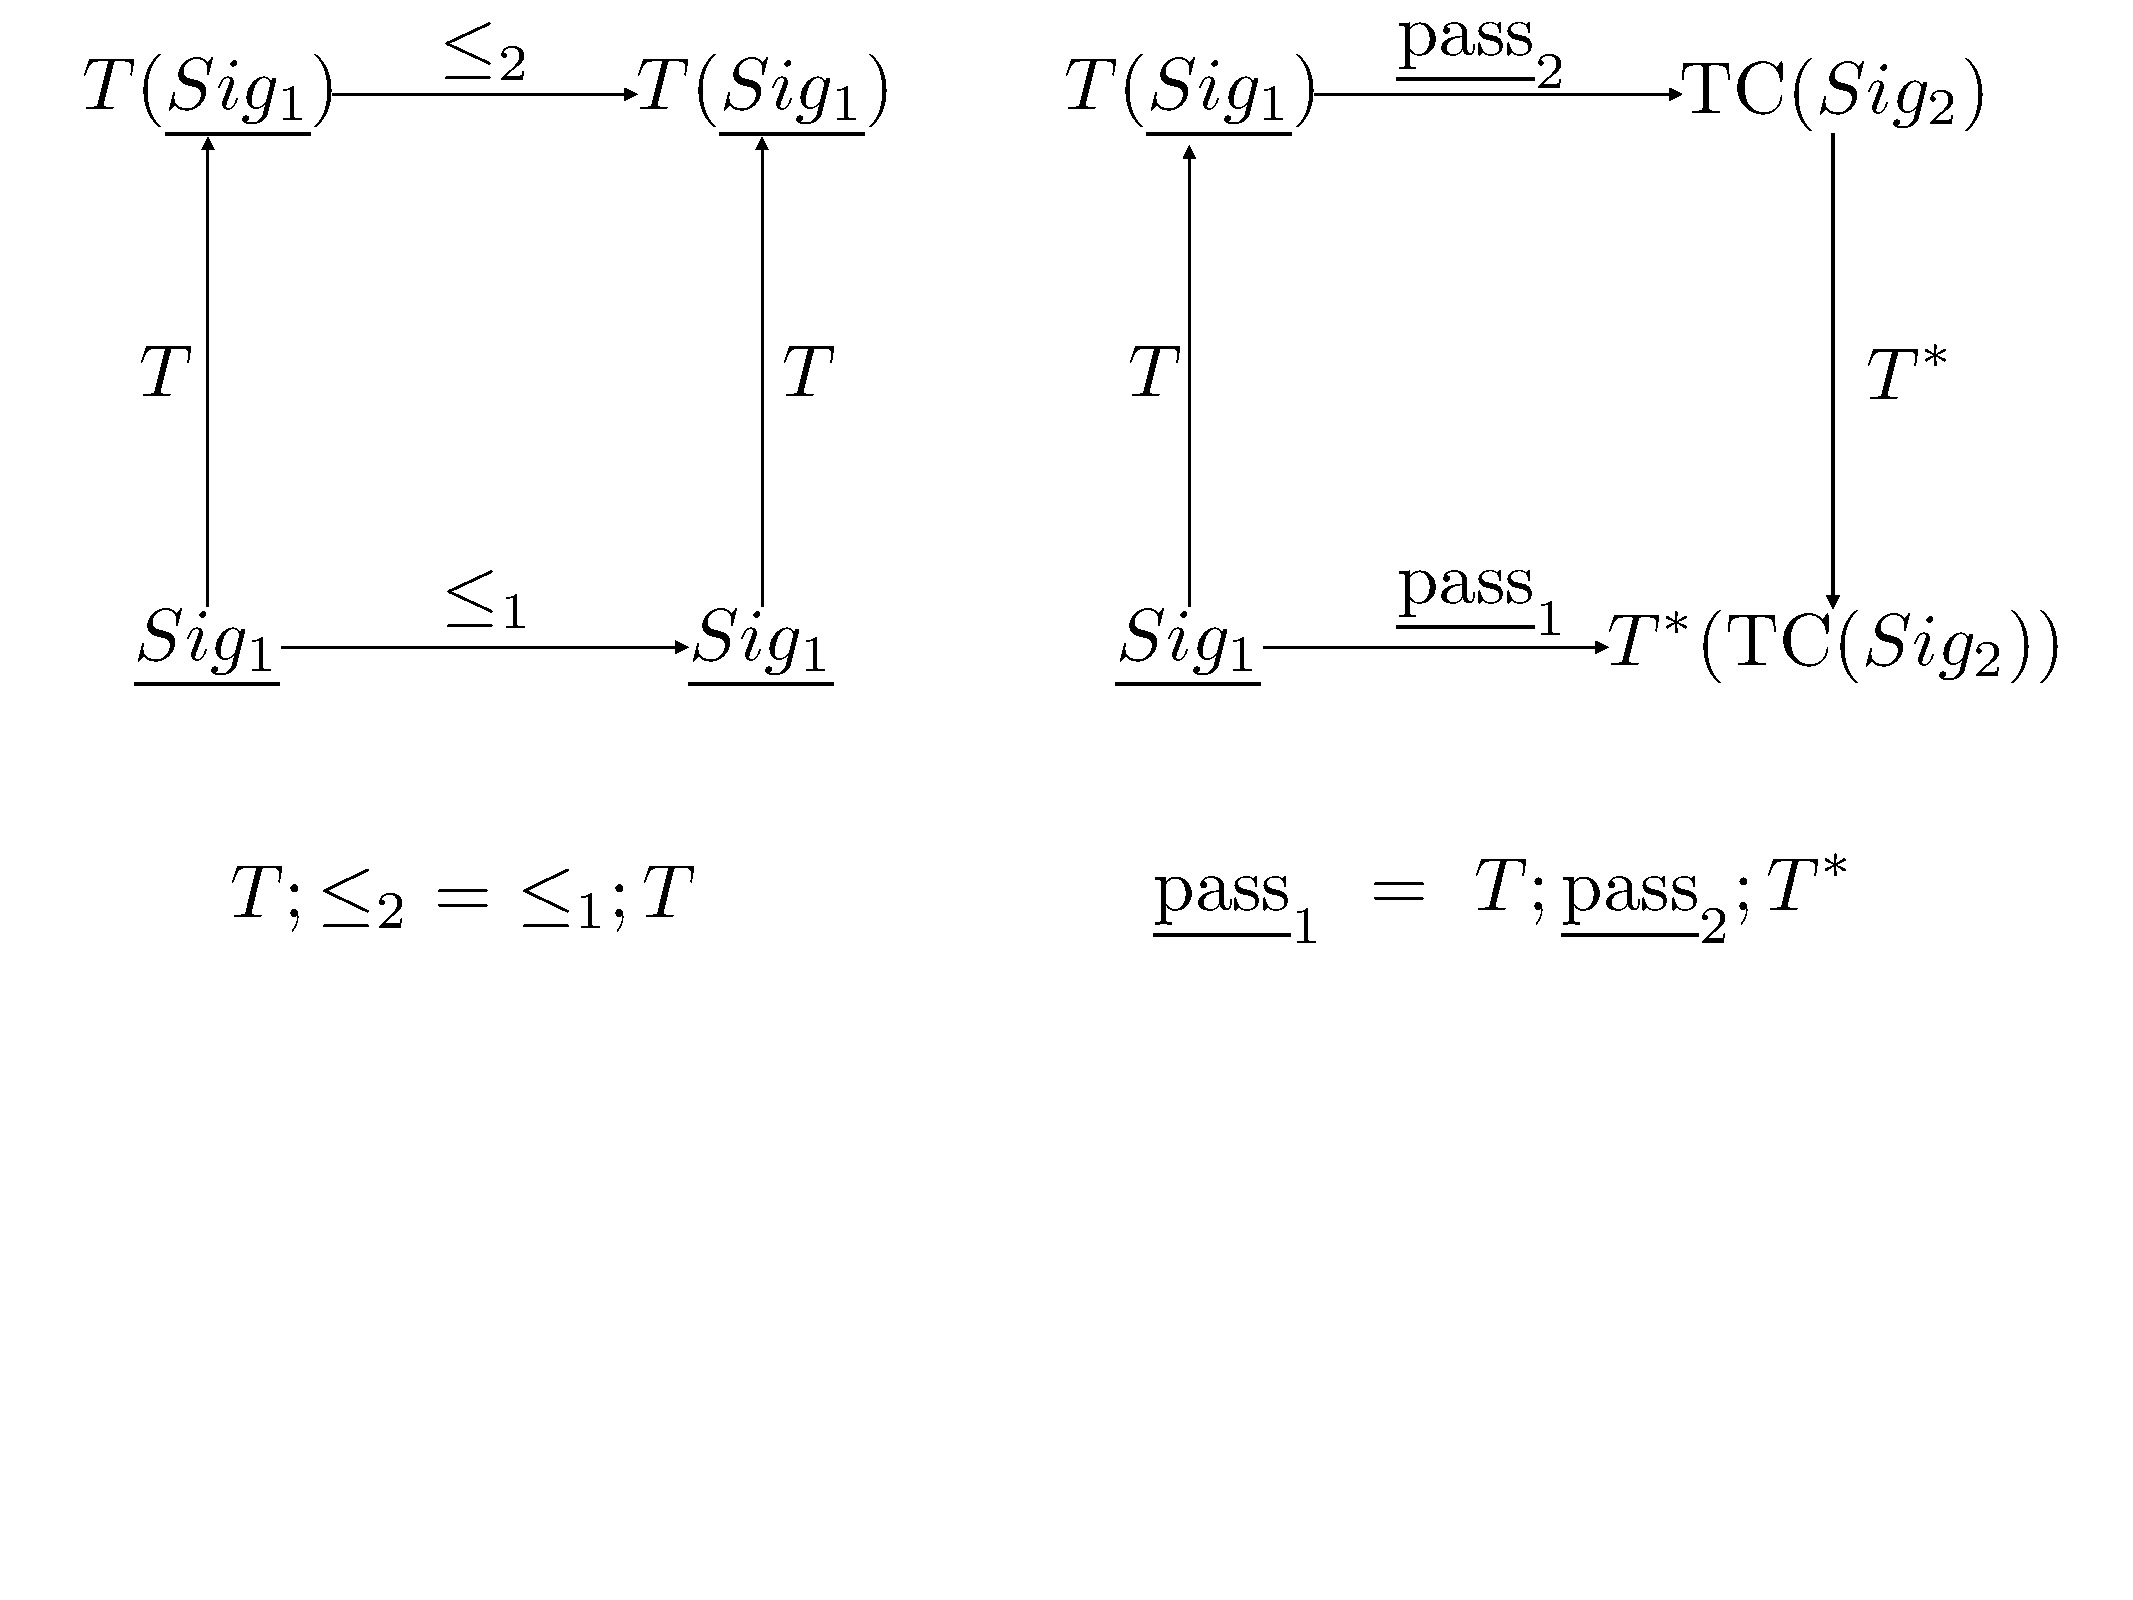
\includegraphics[width=0.6\textwidth]{satisfaction-condition.pdf}
\vspace*{-20mm}
 \caption{Commuting diagrams reflecting the satisfaction condition.}
 \label{fig:satisfaction-relation}
 \end{figure}
% .............................................................................

 

% ============================================================================

 The following theorem is a direct consequence of~\cite[Theorem~2.1]{Huang2017}.

\begin{theorem}\label{th:theorytranslation}
With the notation introduced above, let  $(T,T^*)$ fulfil the satisfaction condition.
Suppose that $\TS_2 \subseteq TC(Sig_2)$ is a complete test suite
for fault model ${\cal F}_2 = ({\cal S}_2,\le_2,Dom_2)$. Define fault model ${\cal F}_1$ on 
$\underline{Sig}_1$ by
$$
{\cal F}_1 = ({\cal S}_1,\le_1,Dom_1),\ \text{such that}\
T({\cal S}_1)  =  {\cal S}_2\ \text{and}\
Dom_1  =  \{ {\cal S}~|~T({\cal S})\in Dom_2 \}.
$$
Then
$$
\TS_1 = T^*(\TS_2)
$$
is a complete test suite with respect to fault model ${\cal F}_1$.
\xbox
\end{theorem}

 
 


% =========================================================================
\subsection{CSP and Refinement}

% -------------------------------------------------------------------------
\subsubsection*{Normalised Transition Graphs}

As shown in~\cite{Roscoe:1994:CME:197600}, any finite-state CSP process $P$ can be represented by a \emph{normalised transition graph} 
$$
G(P) = ( N, \ii n, \Sigma, t : N\times\Sigma \pfun N, a : N \fun \mathbb{P}\mathbb{P}(\Sigma)),
$$
with nodes $N$, initial node $\ii n\in N$, and process alphabet $\Sigma$. The partial \emph{transition function} $t$ maps a node $n$ and an event $e\in\Sigma$ to its successor node $t(n,e)$, if and only if $(n,e)$ are in the domain of $t$. Normalisation of $G(P)$ is reflected 
by the fact that $t$ is a function. The total function $a$ maps each node to its set of \emph{minimal acceptances}: 
if $n\in N$ corresponds to a deterministic process state of $P$, $a(n)$ contains a single acceptance $A\subseteq \Sigma$, and every $e\in A$ is in one-one-correspondence with a transition $t(n,e)$. If $n$ corresponds to a nondeterministic process state, $a(n)$ contains at least two acceptances $A_1, A_2, \dots, A_k$. This reflects the fact that in a nondeterministic state, $P$ must accept all events of one acceptance 
$A_i, i \in \{ 1,\dots,k\}$, but may refuse all events $e$ from 
$A_j \setminus A_i, j\neq i$. 

Each well-defined transition graph $G(P)$ fulfils the following condition. The union of all minimal acceptances in each node corresponds to the set of events labelling its outgoing transitions.
\begin{equation}
\label{eq:wellformedg}
\forall n\in N: (n,e)\in\dom~t \Leftrightarrow e\in\bigcup a(n)
\end{equation}
In this condition, $\dom~t$ denotes the domain of function $t$. 

By construction, normalised transition graphs reflect the failures semantics of finite-state CSP processes: 
the traces $s$ of a process are exactly the paths through the transition graph, 
starting at $\ii n$. The maximal refusals in each process state $P/s$
 are the complements of 
the minimal acceptances of the node $n$ 
corresponding to $P/s$. As a consequences, all failures 
of $P$ are represented by some $(s,R)$, where $s$ is an initialised path through the transition graph and $R\subseteq (\Sigma-A)$ for some minimal acceptance $A\in a(n)$, 
such that $n$ is the node corresponding to $P/s$. 

\begin{example}\label{ex:a}
Consider CSP process 
\begin{eqnarray*}
P & = & a \then (Q\intchoice R)
\\
Q & = & a \then P \extchoice c \then P
\\
R & = & b \then P \extchoice c \then R
\end{eqnarray*}
Its transition graph $G(P)$ is shown in Fig.~\ref{fig:tga}. Process state $P$ is represented there as Node\_0, with $\{ a\}$ as the only acceptance, since event $a$ can never be refused, and no other events are accepted. Having engaged into $a$, the transition emanating from Node\_0 leads to Node\_2 representing  the process state 
$P/a = Q\intchoice R$. The internal choice operator induces several acceptance sets derived from $Q$ and $R$. Since these processes accept their initial events with external choice, 
process $Q\intchoice R$ induces just two minimal acceptance sets $\{a,c\} = [Q]^0$ and
$\{b,c\} = [R]^0$. Note that event $c$ can never be refused, since it is a member of all minimal acceptances. 

Having engaged into $c$, the next process state is represented by Node\_1. Due to normalisation, there was only a single transition satisfying 
$t(\text{Node\_2},c) = \text{Node\_1}$. This transition, however, can have been caused 
by either $Q$ or $R$ engaging into $c$, so Node\_1 corresponds to process state
$Q/c \intchoice R/c = P \intchoice R$. This is reflected by the two minimal acceptances
labelling Node\_1. 
\xbox
\end{example}


% .....................................................................................
 \begin{figure}
 %%\hspace*{-40mm}
 \begin{center}
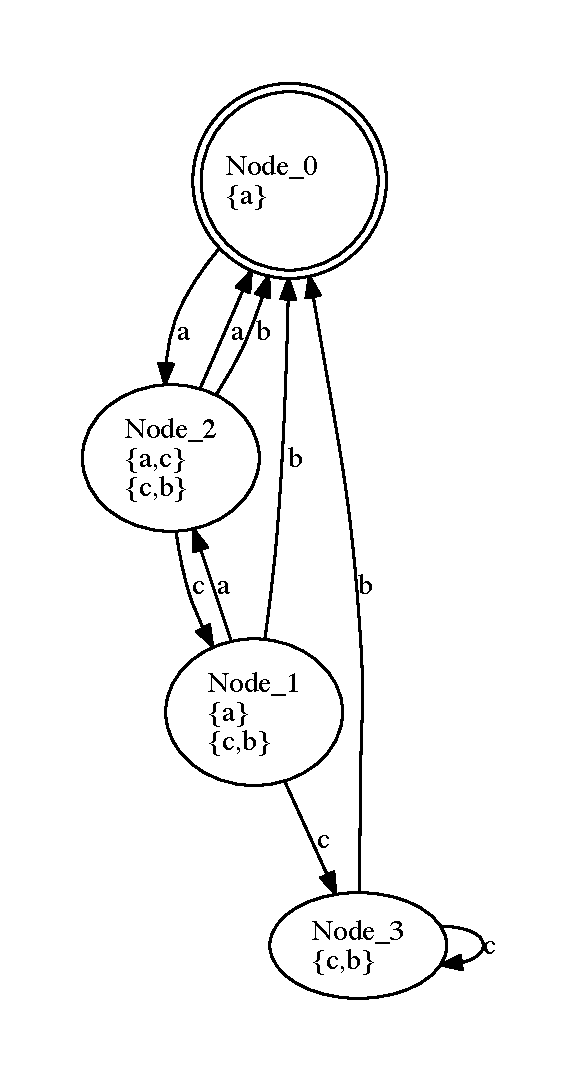
\includegraphics[width=.5\textwidth]{q0.pdf}
\end{center}
%%\vspace*{-10mm}
\caption{Normalised transition graph of CSP process $P$ from Example~\ref{ex:a}.}
 \label{fig:tga}
 \end{figure}
% ....................................................................................... 



% =========================================================================
\subsection{Finite State Machines}

% ==========================================================================
\section{Finite Complete Test Suites for CSP}
\label{sec:finitecomplete}
% ==========================================================================

Here, we present a model map and a test case map pair for CSP processes that
fulfils the satisfaction condition. In Section~\ref{sec:mmap} we present the
model map, and in Section~\ref{sec:tcmap}, the test case map.

% ==========================================================================
\subsection{A Model Map from CSP Processes to Finite State Machines}
\label{sec:mmap}
% ==========================================================================

We now construct a model map for associating CSP processes represented by
normalised transition graphs to finite state machines. The intuition behind
this construction is that the finite state machine's input alphabet
corresponds to {\it sets of inputs} that may be offered to a CSP process.
Depending on the events contained in this set, the process may (1)~accept all
of them, (2)~accept some of them while refusing others, or (3)~refuse all of
them. This is reflected in the FSM by outputs   representing events that the
process really has engaged in and an extra event $\bot$ representing refusal,
if the set of events has been blocked. In the FSM, blocked sets of events are
always associated with self-loop transitions: the state is not changed,
because the corresponding CSP process also remains blocked in its current
state if it refuses an event.

More formally, we a finite alphabet $\Sigma$ of events and consider a
finite-state process $P$ (with events in this alphabet) with normalised
transition graph $G(P)=( N, \ii n, \Sigma, t : N\times\Sigma \pfun N, r : N
\fun \mathbb{P}\mathbb{P}(\Sigma))$. The model map $T$ maps $P$ to the
following observable FSM $T(P) = (Q,\ii q, \Sigma_I,\Sigma_O,h)$ specified by
%
\begin{eqnarray*}
  Q & = & N
  \\
  \ii q & = & \ii n
  \\
  \Sigma_I & = & \power(\Sigma) - \{ \varnothing \}
  \\
  \Sigma_O & = & \Sigma \cup \{ \bot\}
  \\
  h & = & \{ (n,A,e,n')~|~A\in \Sigma_I \wedge e\in A \wedge (n,e)\in \dom~t\wedge t(n,e) = n' \} \cup
  \{ (n,A,\bot,n)~|~A\in r(n) -\{\varnothing\} \}
\end{eqnarray*}
%
We say that FSM trace $(x/s) \in L(T(P))$ and CSP trace $s'\in\text{tr}(P)$
are \emph{corresponding traces}, if $s' = s\project \Sigma$. Observe that the
FSM output trace $s$ may contain deadlock events $\bot$ that are not
contained in the  process alphabet $\Sigma$. So, we have corresponding traces
if they only differ by the presence or absence of $\bot$. 

% ...................................................................................
 \begin{figure}
 %%\hspace*{-40mm}
 \begin{center}
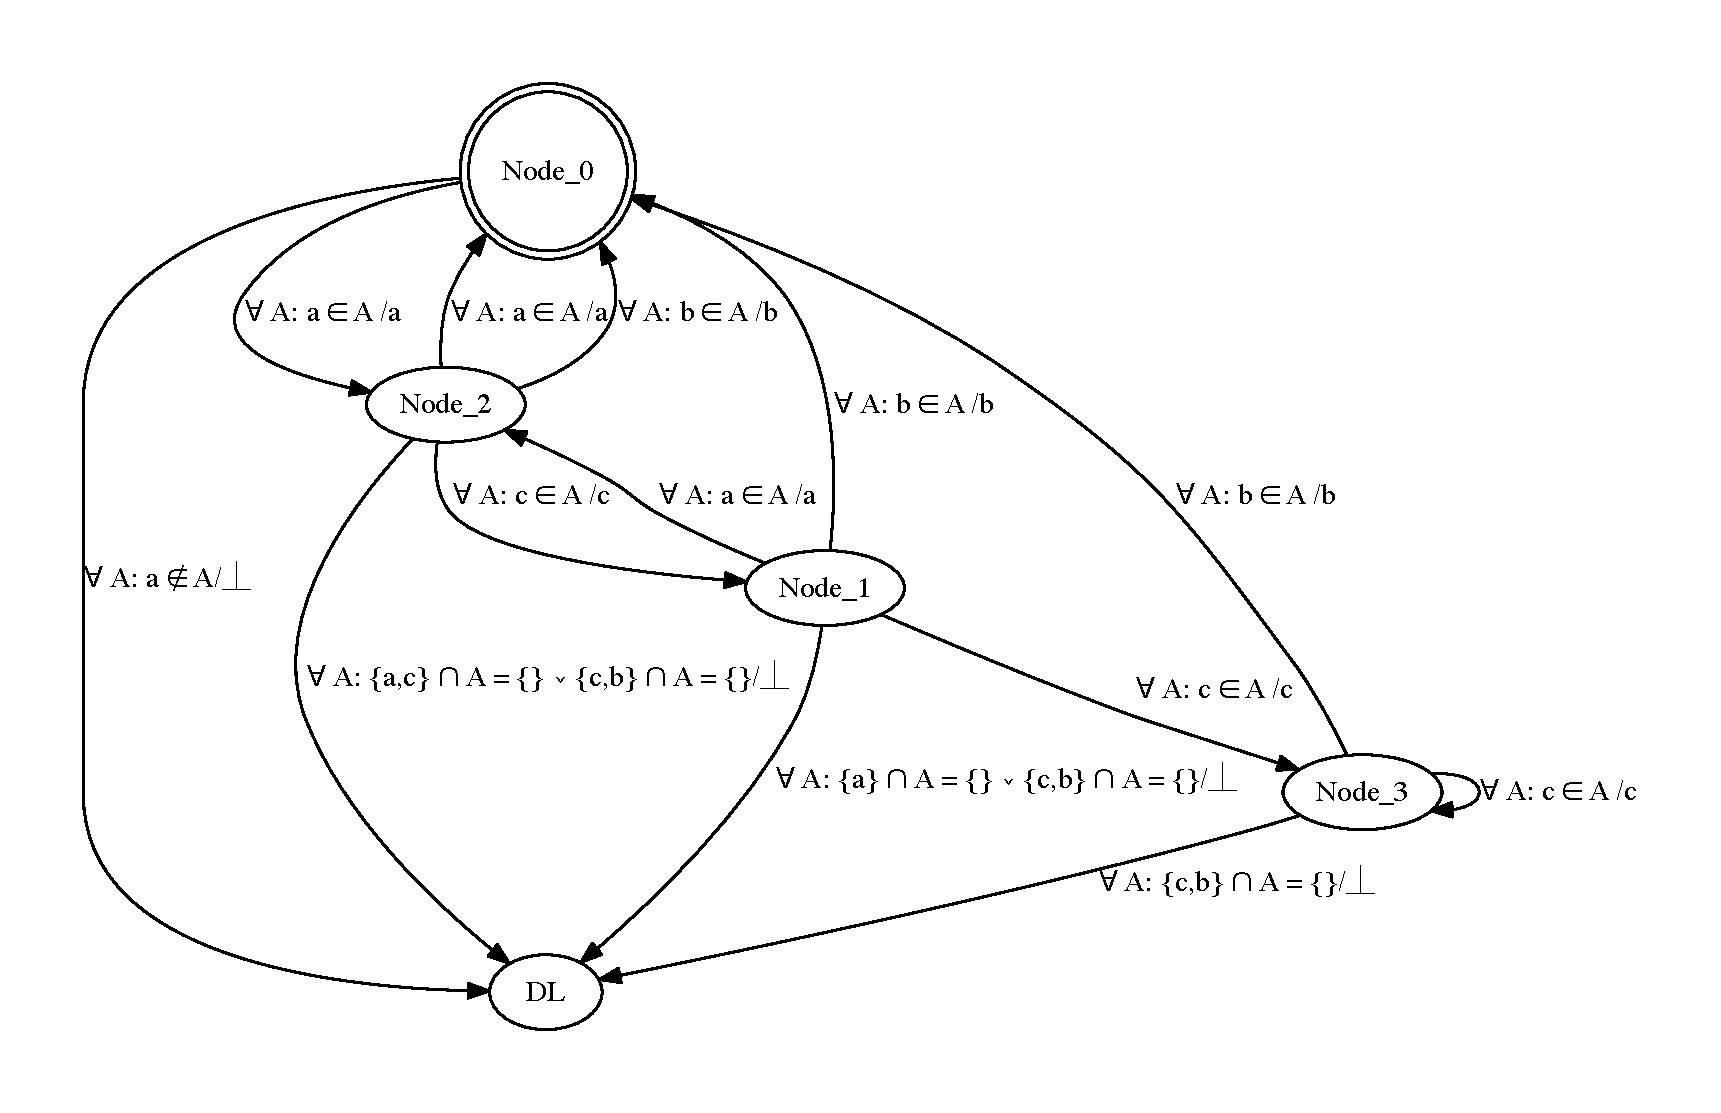
\includegraphics[width=\textwidth]{fsm0.pdf}
\end{center}
%%\vspace*{-10mm}
\caption{FSM resulting from applying the model map to CSP process $P$ from Example~\ref{ex:a}.}
 \label{fig:fsm0}
 \end{figure}
% ...................................................................................


\begin{example}{ex:b}
For the CSP process $P$ and its transition graph $G(P)$ discussed in Example~\ref{ex:a}, the FSM $T(P)$ is depicted in Fig.~\ref{fig:fsm0}.
For displaying its transitions, we used notation
$$
(\text{condition}(A)) / e
$$
which stands for a set of transitions between the respective nodes: one transition per non-empty set $A\subseteq \Sigma$ fulfilling the specified condition.
The arrow
$$
\text{Node\_0} \xrightarrow{(a\in A) / a} \text{Node\_2},
$$
for example, stands for FSM transitions
$$
\begin{array}{l}
\text{Node\_0} \xrightarrow{\{a\}/a} \text{Node\_2} \\
\text{Node\_0} \xrightarrow{\{a,b\}/a} \text{Node\_2} \\
\text{Node\_0} \xrightarrow{\{a,c\}/a} \text{Node\_2} \\
\text{Node\_0} \xrightarrow{\{a,b,c\}/a} \text{Node\_2} \\
\end{array}
$$
\end{example}


We are now in the position to state and prove the theorem about the model map
fulfilling the satisfaction condition {\bf SC1} introduced in Section~\ref{sec:transltt}. To this end, we first introduce five lemmas.


\begin{lemma}\label{tran}
Let $s\in \trc(P)$ and $n=G(P)/s$ be the node of $G(P)$ corresponding the process state $P/s$.
Then for any $x\in \Sigma_I$, $y\in \Sigma_O\colon$
\begin{align*}(n,x,y,n')\in h\Leftrightarrow &(y\in x\wedge s.y\in \trc(P)\wedge n'=G(P)/s.y)\vee\\ &(y=\bot \wedge (s,x)\in {\text {\rm Fail}}(P)\wedge n'=n)\end{align*}
\end{lemma}

\begin{proof}
Let $s'=s.y\project \Sigma$.
We consider the following two cases:
\begin{itemize}
\item[1.] Suppose $y=e$ for some $e\in \Sigma$. Then $s'=s.e$. By definition of $h$, we have
\begin{align*}(n,x,e,n')\in h\Leftrightarrow & e\in x\wedge (n,e)\in {\text{\rm dom}}\, t\wedge n'=t(n,e)\\ \Leftrightarrow& e\in x\wedge s.e\in \trc(P)\wedge n'=G(P)/s.e\end{align*}
\item[2.] Suppose $y=\bot$. Then $s'=s$, and we can derive
\begin{align*}(n,x,\bot,n')\in h\Leftrightarrow & x \in {\text {\rm Ref}}(P/s)\wedge n'=n \\
\Leftrightarrow & (s,x) \in {\text {\rm Fail}}(P)\wedge n'=n\end{align*}
\end{itemize}
\end{proof}

%%----------------------------------------------------------------------------
%-----------------------------------------------------------------------------

\begin{lemma}\label{trac}

Let $x/y\in (\Sigma_I\times\Sigma_O)^*$ and $s=y\project \Sigma$. Then $$x/y\in L(T(P))\Rightarrow s\in\trc(P) \wedge \underline q\after x/y=G(P)/s.$$
\end{lemma}
\begin{proof}
We prove the lemma by induction on $\#(x/y)$,  the length of $x/y$. For the base case, suppose that $x/y=\varepsilon $, then $s=\varepsilon $ and $\underline q\after x/y=\underline n=G(P)/{\varepsilon }$. For the induction hypothesis, suppose the statement holds for all $x/y\in (\Sigma_I\times\Sigma_O)^*$ with $\#(x/y)=k$, for some $k\ge 0$. Let $x/y\in (\Sigma_I\times\Sigma_O)^*$ with $\#(x/y)=k$ and $x'/y'\in \Sigma\times \Sigma_O$. To perform the induction step, let $y\project \Sigma=s$ and $y.y'\project \Sigma=s'$. Then by the induction hypothesis we have $s\in\trc(P)$ and $\underline q\after x/y=G(P)/s$.
Since $x.x'/y.y'\in L(T(P))$, there is a transition $(G(P)/s',x',y',n)\in h$ and $n=\underline q\after x/y$. By Lemma~\ref{tran} we have $s'=s.y'\in \trc(P)\wedge \underline q\after x.x'/y.y'=G(P)/s'$.
\end{proof}%-----------------------------------------------------------------------------

%-----------------------------------------------------------------------------

\begin{lemma}\label{exte}
Let $x/y\in (\Sigma_I\times \Sigma_O)^*$ and $x/y\in L(T(P))$. Let $x'/y'\in \Sigma_I\times \Sigma_O$. Then
\begin{eqnarray*}
x.x'/y.y'\in L(T(P)) & \Leftrightarrow  &
\big(y'\in x'\wedge (y.y')\project \Sigma\in \trc(P)\big)\vee {}
\\ & & \big(y'=\bot\wedge (y\project \Sigma, x')\in {\text {\rm Fail}}(P)\big).
\end{eqnarray*}
\end{lemma}

\begin{proof}
Let $x/y\in (\Sigma_I\times \Sigma_O)^*$ and $x/y\in L(T(P))$. Let $x'/y'\in \Sigma_I\times \Sigma_O$. Then by Lemma~\ref{trac}, we have $s=y\project \Sigma\in \trc(P)$ and $G(P)/s=\underline q\after x/y$. From Lemma~\ref{tran} we have the following:
\[\begin{array}{lll}
&&x.x'/y.y'\in L(T(P)) \\&\Leftrightarrow & \exists n'\in Q: (G(P)/s,x',y',n')\in h\\
&\Leftrightarrow & (y'\in x'\wedge s.y'\in \trc(P))\vee (y'=\bot\wedge (s, x')\in {\text {\rm Fail}}(P)\big)\\
&\Leftrightarrow & (y'\in x'\wedge (y.y')\project \Sigma\in \trc(P)\big)\vee \big(y'=\bot\wedge (y\project \Sigma, x)\in {\text {\rm Fail}}(P)\big)\end{array}
\]
\end{proof}


%----------------------------------------------------------------------------
%----------------------------------------------------------------------------
\begin{lemma}\label{cont}
For any $s\in \Sigma^*$,
$$s\in \trc(P) \Leftrightarrow \exists x\in \Sigma_I^*: x/s \in L(T(P)).$$
\end{lemma}
%
%--------------------------------------------------------------------------------------------------
\begin{proof}
Let $s\in \Sigma^*$. We prove the lemma by induction on $\#s$ the length of $s$. Suppose $s=\varepsilon $, then $s\in \trc(P)\wedge x=\varepsilon \Leftrightarrow x/s\in L(T(P))$. Suppose the statement holds for all $s\in \Sigma^*$ with $\#s=k$, for some $k\ge 0$. Let $s\in \Sigma^*$ with $\#s=k$ and $e\in\Sigma$.
Then \[\begin{array}{llll}
&& s.e\in \trc(P)\\
&\Leftrightarrow & s\in \trc(P)\wedge s.e\in \trc(P)\\
&\Leftrightarrow &  \exists x\in \Sigma_I^*: x/s\in L(T(P))\wedge s.e\in \trc(P)\\
&\Rightarrow & \exists x\in \Sigma_I^*: x.\{e\}/s.e\in L(T(P))&[{\text{Lemma~\ref{exte}}}]\\
&\Rightarrow & \exists x\in \Sigma_I^*: x/s.e\in L(T(P))
\end{array}
\]
 \[\begin{array}{llll}
&& \exists x\in \Sigma_I^*: x/s.e\in L(T(P))\\
&\Leftrightarrow & \exists x\in \Sigma_I^*\wedge \exists x'\in \Sigma_I: x/s\in L(T(P))\wedge x.x'/s.e\in L(T(P))\\
&\Rightarrow & s.e\in \trc(P)&[{\text{Lemma~\ref{exte}}}]\\
\end{array}
\]
\end{proof}
%----------------------------------------------------------------------------

%---------------------------------------------------------------------------
\begin{lemma}\label{conf}
For any $s\in \Sigma^*$ and $x'\in \Sigma_I$,
$$(s,   x')\in {\text {\rm Fail}}(P)\Leftrightarrow \exists x\in \Sigma_I^*: x.x'/s.\bot \in L(T(P))$$
\end{lemma}
\begin{proof}
$\forall s\in \Sigma^*, x'\in \Sigma_I$:
\[\begin{array}{llll}
&& \exists x\in \Sigma_I^*: x.x'/s.\bot\in L(T(P))&\\
&\Leftrightarrow & \exists x\in \Sigma_I^*: x/s\in L(T(P))\wedge x.x'/s.\bot\in L(T(P))&\\
&\Leftrightarrow & (s,   x')\in {\text {\rm Fail}}(P)&[{\text {Lemma~\ref{exte} and ~\ref{cont}}}]

\end{array}
\]
\end{proof}
%------------------------------------------------------------------------------
\begin{theorem}
Let $P,Q$ be two CSP processes over the same alphabet $\Sigma$. Then\\
$T(Q)\preceq T(P) \Leftrightarrow P\,\sqsubseteq_F\, Q$
\end{theorem}
\begin{proof}
Suppose $T(Q)\preceq  T(P)$. Let $s\in \Sigma^*, x'\in \Sigma_I$. Then by Lemma~\ref{cont} and Lemma~\ref{conf}

\[\begin{array}{lll}
 s\in \trc(Q) &\Leftrightarrow & \exists x\in \Sigma_I^*: x/s\in L(T(Q))\\
&\Rightarrow& \exists x\in \Sigma_I^*:  x/s\in  L(T(P))\\
&\Leftrightarrow &s\in \trc(P)\\
\end{array}
\]

\[\begin{array}{lll}
(s,   x')\in {\text {\rm Fail}}(Q) &\Leftrightarrow & \exists x\in \Sigma_I^*: x.x'/s.\bot \in L(T(Q))\\
&\Rightarrow& \exists x\in \Sigma_I^*: x.x'/s.\bot \in L(T(P))\\
&\Leftrightarrow &(s,   x')\in {\text {\rm Fail}}(P)\\
\end{array}
\]

Hence $$T(Q)\preceq  T(P)\Rightarrow P\,\sqsubseteq_F\, Q$$

Now suppose $P\,\sqsubseteq_F\, Q$. We prove by induction on $\#(x/y)$ that for any $x/y\in (\Sigma_I\times \Sigma_O)^*$,  $x/y\in L(T(Q))\Rightarrow x/y\in L(T(P))$ holds.
It is trivial if $\#(x/y)=0$. Suppose $x/y\in L(T(Q))\Rightarrow x/y\in L(T(P))$ holds for any $x/y\in (\Sigma_I\times \Sigma_O)^*$ of length $k\ge 0$.
For any $x/y\in (\Sigma_I\times \Sigma_O)^*$ of length $k$ and for any   $x'/y'\in \Sigma_I\times \Sigma_O$. Let $s=y\project \Sigma$ and $s'=(y.y')\project \Sigma$. Then by Lemma~\ref{exte} and $ P\,\sqsubseteq_F\, Q$ we have
\[\begin{array}{lll}
&&x.x'/y.y'\in L(T(Q))\\&\Rightarrow& x/y\in L(T(Q))\wedge \big((y'\in x'\wedge s'\in \trc(Q))\vee (y'=\bot\wedge (s, x)\in {\text {\rm Fail}}(Q))\big)\\
&\Rightarrow& x/y\in L(T(P))\wedge \big((y'\in x'\wedge s'\in \trc(P)\big)\vee (y'=\bot\wedge (s, x)\in {\text {\rm Fail}}(P))\big)\\
 &\Rightarrow& x.x'/y.y'\in L(T(P)) \\
\end{array}
\]
Hence $$ P\,\sqsubseteq_F\, Q \Rightarrow T(Q)\preceq  T(P)$$.
\end{proof}


% ==========================================================================
\subsection{A Test Case Map from Finite State Machines to CSP Processes}
\label{sec:tcmap}

% -------------------------------------------------------------------------
\subsubsection*{FSM Test Cases}

Following~\cite{DBLP:conf/hase/PetrenkoY14},
an \emph{adaptive FSM test case}
$$
tc_\text{FSM}=(Q,\ii q,\Sigma_I,\Sigma_O,h,in)
$$
is a nondeterministic, observable, output-complete, acyclic FSM which only provides a single input in a given state. Running in FSM intersection mode with the SUT, the test case provides a specific input to the SUT; this input is determined by the current state of the test case. It accepts every output and transits either to a fail-state FAIL, if the output is wrong according to the test objectives, or to the next test state uniquely determined  by the processed input/output pair. Another state PASS indicates that
the test has been completed without failure. Both FAIL and PASS are termination states, that is, they do not have any outgoing transitions.

Since the test case state determines the input for all of its outgoing transitions, this input is typically used as a state label, and the outgoing transitions are just labelled by the possible outputs. A function $in : Q -\{  \text{PASS}, \text{FAIL} \}
\fun\Sigma_I$ maps the states to these inputs. Termination states
of the FSM are not labelled with further inputs.

There is no requirement that an FSM test case running in intersection mode against
an FSM $M$ acting as SUT should {\it always} reach the PASS state. Since the SUT may be nondeterministic, it may perform a joint test execution that blocks before
the test case's PASS state is reached. In such a case, the result of the test execution is \emph{inconclusive}. Due to nondeterminism, for $M$ to pass a test case, it
has to checked that {\it every possible} test execution of  $tc_\text{FSM}$ against $M$
terminates either in PASS, or that the result remains inconclusive. If one execution ends in FAIL, the test verdict is FAIL. More formally,
$$
M\ \pass\ tc_\text{FSM} \equiv
\big(
\forall x/y \in L(M)\cap L(tc_\text{FSM}): \ii q\after(x/y) \neq FAIL
\big).
$$

\begin{example}{ex:xx}
Consider the FSM test case depicted in Fig.~\ref{fig:fsm0tc} which is specified
for the same input and output alphabets as defined for  the FSM presented in Example~\ref{ex:b}. The test case is passed by the FSM from Example~\ref{ex:b}, because
intersecting the two state machines results in an FSM which always reaches the PASS state.
\end{example}


% ...................................................................................
 \begin{figure}
 %%\hspace*{-40mm}
 \begin{center}
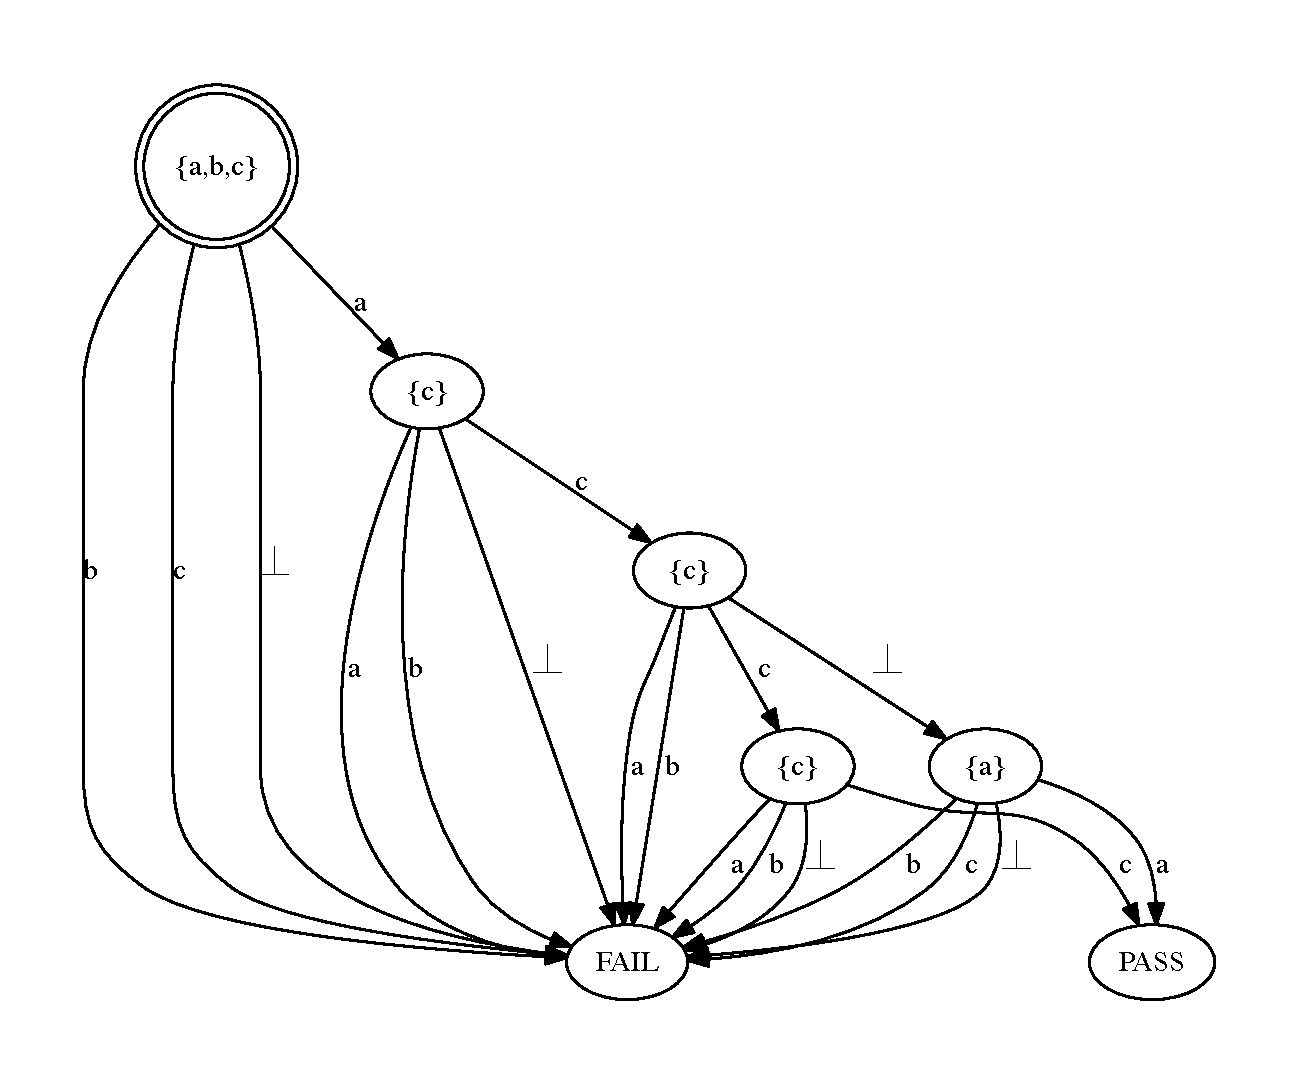
\includegraphics[width=.8\textwidth]{fsm0tc.pdf}
\end{center}
%%\vspace*{-10mm}
\caption{An FSM test case which is passed by the FSM presented in Example~\ref{ex:b}.}
 \label{fig:fsm0tc}
 \end{figure}
% ...................................................................................




% -------------------------------------------------------------------------
\subsubsection*{CSP Test Cases}
\label{sec:csptc}
A \emph{CSP test case} $tc_\text{CSP}$  is a terminating process with alphabet
$\Sigma\cup\{\dag,\bot,\tick \}$, where the extra events stand for
(1) test  verdict FAIL ($\dag$), (2) timeout ($\bot$), and (3) test
 verdict PASS ($\tick$). The test case runs in parallel with the SUT $P$,
 synchronising over all events from the visible alphabet $\Sigma$ of $P$. This is
 expressed by the formula
 $$
 P\parallel[\Sigma] tc_\text{CSP}.
 $$

 In analogy to FSM test cases, a CSP process $P$ passes a test case $tc_\text{CSP}$
 if the traces of the parallel composition do not contain the failure event, that is,
 $$
 P\ \pass\ tc_\text{CSP} \equiv \big(
 \forall s\in\trc(P\parallel[\Sigma] tc_\text{CSP}): (s\project \{\dag\}) = \varepsilon
 \big)
 $$


 In principle, very general classes of CSP processes can be
 used for testing, as introduced, for example,
 in~\cite{DBLP:conf/fm/PeleskaS96,peleska1997a}. For the purpose of this paper, however, we can restrict the possible variants of CSP test cases to the ones that are in the range of the test case map which is constructed next.


% -------------------------------------------------------------------------
\subsubsection*{Test Case Map}

The test case map $T^* :TC(FSM) \fun TC(CSP)$ is specified with respect to a fixed
CSP process alphabet $\Sigma$ extended by the events $\{\dag,\bot,\tick \}$ introduced
above
and the associated FSM input and output alphabets
$\Sigma_I = \power(\Sigma)-\{\varnothing\}$ and $\Sigma_O=\Sigma\cup \{\bot \}$.
Given an FSM test case $tc_\text{FSM}=(Q,\ii q,\Sigma_I,\Sigma_O,h,in)$,
the image $T^*(tc_\text{FSM})$ is the CSP process $tc_\text{CSP}$ specified
as follows.
\begin{eqnarray*}
tc_\text{CSP} & = & tc(\ii q)
\\
tc(q) & = & \big( e :  A(q) \then  tc(q\after (in(q)/e)) \big)
\\ & & \extchoice
 \big( e : A_\text{PASS}(q)   \then \tick \then \Skip \big)
\\ & & \extchoice
 \big( e : A_\text{FAIL}(q) \then \dag \then \Skip \big)
\\ & &
\\
A(q) & = & \{ a\in in(q)\cup\{\bot\}~|~q\after (in(q)/a)\notin \{\text{PASS},\text{FAIL}\} \}
\\
A_\text{PASS}(q) & = & \{ a\in in(q)\cup\{\bot\}~|~q\after(in(q)/a) = \text{PASS} \}
\\
A_\text{FAIL}(q) & = & \{ a\in in(q)\cup\{\bot\}~|~q\after(in(q)/a) = \text{FAIL} \}
\end{eqnarray*}

Intuitively speaking, $tc_\text{CSP}$ offers in each test step the same events to
the CSP process to be tested as the FSM test case offers to the FSM under test.
These events are specified in each non-terminating test step by $in(q)$, where
$q$ is the current state of the FSM test case $tc_\text{FSM}$. While the FSM test
case offers these events a single set-valued member of the input alphabet $\Sigma_I$
to the FSM under test, the CSP test offers the same to the SUT by means of an external choice, so that it just depends on the SUT which event to choose. In addition to the
events from $in(q)$, the CSP test case
accepts the event $\bot$ which is not shared with
the SUT but represents a timeout event provided by the testing environment to indicate
that the SUT is blocked without accepting any of the events in $in(q)$.

The events offered/accepted by the CSP test in state $tc(q)$ are partitioned into
3 sets $A(q)$, $A_\text{PASS}(q)$, and $A_\text{FAIL}(q)$. The disjointness of these
sets is a consequence of the fact that the FSM test case is observable: if
$tc_\text{FSM}$ can transit, for example, from $q$ to FAIL with I/O $in(q)/a$,
then there exists no other transition from $q$ which is also
labelled by $in(q)/a$.



% ..........................................................................
\begin{example}{ex:zz}
The FSM test case $tc_\text{FSM}$
shown in Fig.~\ref{fig:fsm0tc} is mapped by $T^*$ to the following
CSP test case.
\begin{eqnarray*}
T^*(tc_\text{FSM}) & = & P_1
\\
P_1 & = & \big(e:\{ b,c,\bot \} \bullet e \then \dag\then\Skip\big)
\extchoice
 \big( a \then P_2 \big)
\\
P_2 & = & \big( e : \{ a,b,\bot \}\bullet e\then \dag\then\Skip  \big)
\extchoice
\big( c\then P_3 \big)
\\
P_3 & = & \big( e : \{ a,b \}\bullet e\then \dag\then\Skip  \big)
\extchoice
\big( \bot \then P_4 \big)
\extchoice
\big( c\then P_5 \big)
\\
P_4 & = & \big( e : \{ b,c,\bot \}\bullet e\then \dag\then\Skip  \big)
\extchoice
\big( a\then\tick\then \Skip \big)
\\
P_5 & = & \big( e : \{ a,b,\bot \}\bullet e\then \dag\then\Skip  \big)
\extchoice
\big( c\then\tick\then \Skip \big)
\end{eqnarray*}
\end{example}

The following theorem shows the validity of the satisfaction condition {\bf SC2}
regarding the test case map, the model map, and the pass conditions for tests on CSP level and FSM level.

% ----------------------------------------------------------------------
\begin{theorem}
Fixing a CSP process alphabet $\Sigma$, the model map
$T : \underline{Sig}_1 \fun FSM$ and the test case map $T^*:TC(FSM) \fun TC(CSP)$ fulfil satisfaction condition {\bf SC2} in the sense that
$$
\forall P\in \underline{Sig}_1, tc_\text{FSM}\in TC(FSM): T(P)\ \pass_2\ tc_\text{FSM} \Leftrightarrow
P\ \pass_1\ T^*(tc_\text{FSM})
$$
\end{theorem}
\begin{proof}
Let $T(P) = (Q,\ii q,\Sigma_I,\Sigma_O,h)$ and
$tc_\text{FSM} = (Q',\ii q',\Sigma_I,\Sigma_O,h',in)$.
We show by induction over the length of $s\in\Sigma_O^*$ that the following
assertions hold for all $s$.
\begin{enumerate}
\item For every pass-trace $x/s \in L(T(P)) \cap L(tc_\text{FSM})$,
there exists a pass-trace $u \in \text{tr}(P\parallel[\Sigma] T^*(tc_\text{FSM}))$, such that
$u\project\Sigma$ corresponds to $x/s$.

\item For every fail-trace  $x/s \in L(T(P)) \cap L(tc_\text{FSM})$,
there exists a fail-trace trace
$u \in \text{tr}(P\parallel[\Sigma] T^*(tc_\text{FSM}))$, such that
$u\project\Sigma$ corresponds to $x/s$.

\item For all $x/s\in L(T(P))$,
the graph nodes of $G(P)$ and the states of $T(P)$ are related by
$$
\begin{array}{l}
G(P)/(s\project\Sigma) = \ii q\after (x/s).
\end{array}
$$

\item FSM test $tc_\text{FSM}$ and CSP test $T^*(tc_\text{FSM})$ perform consistent
state changes, in the sense that
$$
\begin{array}{l}
x/s\in L(T(P))\cap L(tc_\text{FSM}) \wedge  \ii q'\after (x/s) \not\in \{\text{PASS},\text{FAIL}\}
\Rightarrow {}
\\\tabd
T^*(tc_\text{FSM})/(s\project \Sigma) = tc(\ii q'\after (x/s)),
\end{array}
$$
where $tc(q)$ has been defined above with the test case map.

\end{enumerate}

Proof of 1 and 2 obviously proves the theorem; assertions~3 and 4 are
needed to perform the induction argument.



For the base case, $s$ is the empty trace $\varepsilon$, so $x/s$ is empty as well. We have
$G(P)/\varepsilon = \ii n = \ii q$, due to the definition of the model map; this proves Assertion~3 for the base case.
FSM test case $tc_\text{FSM}$ resides in its initial state $\ii q'$. By definition of the test case map above, $T^*(tc_\text{FSM})$ has initial CSP process state $tc(\ii q')$; this proves  Assertion~4 for the base case $\#s = 0$. For assertions 1 and 2, there is nothing to
prove: no test can pass or fail on the empty trace.

For the induction hypothesis, assume that the four assertions have been proven for
$\#s \le k$ with $0\le k$.

For the induction step, assume that the FSM $T(P)$
has run through trace $x/s\in L(T(P))\cap L(tc_\text{FSM})$ such that
$\#s \le k$ and $\ii q\after(x/s) = q\in N$. Moreover, the FSM test case
$tc_\text{FSM}$ fulfils  $\ii q'\after (x/s) = q'$ for a uniquely defined state
$q'\in Q'$. The induction hypothesis gives us
$G(P)/(s\project\Sigma) = \ii q\after (x/s) = q$
from Assertion~3 and
$T^*(tc_\text{FSM})/(s\project \Sigma) = tc(q')$ from Assertion~4.
FSM test $tc_\text{FSM}$ will offer input $in(q')$ to the FSM $T(P)$ which is being tested. We distinguish two cases  for the outcomes of the resulting test step.


\medskip
\noindent
{\bf Case~1.} $(x.in(q'))/(s.\bot) \in L(\ii q\after (x/s))$.\newline
By construction of $T(P)$, this is exactly the case if
$in(q')\in r(G(P)/(s\project \Sigma)) - \{ \varnothing\}$. By construction of $T(P)$,
this FSM will perform a self-loop transition labelled by $in(q')/\bot$ and therefore remain in $q$. For $P$, the corresponding behaviour is to refuse all events from
$in(q')$, so $q$ also remains as the current state in $G(P)/(s\project \Sigma)$. This proves Assertion~3 for the induction step, Case~1.

Since $tc_\text{FSM}$ is output complete,
$in(q')/\bot \in L(q')$. Depending on the nature of the test case,
$q'\after (in(q')/\bot)$ is one of the deadlock states PASS, FAIL, or it is a
non-blocking FSM state, say, $q''$. Since $tc_\text{FSM}$ is observable, however,
this post-state is uniquely determined.
Since the sets $A(q)$, $A_\text{PASS}(q)$, and $A_\text{FAIL}(q)$
are disjoint,   $T^*(tc_\text{FSM})$
has exactly one choice to proceed and will come to the post-states that are analogous to those of $tc_\text{FSM}$: if $tc_\text{FSM}$ terminates in PASS(FAIL), then
$T^*(tc_\text{FSM})$ will produced the events $\bot$ followed by
$\tick(\dag)$ and terminate. If $tc_\text{FSM}$  transits with $in(q)/e$ to $q''$, CSP test case
$T^*(tc_\text{FSM})$ will perform $e\in A(q)$ as well and continue like process
$tc(q'\after(in(q')/\bot)$ with $q'\after(in(q')/\bot) = q''$.
Since $\bot,\tick,\dag$ are not contained in $\Sigma$, the CSP process $P$
cannot block these transitions of  $T^*(tc_\text{FSM})$, since we have assumed $P$ to be non-divergent. This shows that $tc_\text{FSM}$ and $T^*(tc_\text{FSM})$ engage into the same pass/fail/continue step, as was to be shown. This proves assertions~1,2,4
for Case~1.




\medskip
\noindent
{\bf Case~2.} $(x.in(q'))/(s.e) \in L(\ii q\after (x/s))$ with $e\in in(q')\subseteq\Sigma$.\newline
By construction of $T(P)$, this case applies whenever $e\in A\wedge (n,e)\in\dom~t$.
Also by construction, FSM $T(P)$ will transit to $t(q,e)$ (recall that
$q = G(P)/(s\project \Sigma)$, so
$q\after(in(q')/e) = u$ for a uniquely defined state $u= t(q,e) \in N$. Since
$G(P)/(s\project \Sigma)$ will also transit to $u$ by definition of $t$, this proves the induction step for Assertion~3.

With the same argument as in Case~1, we conclude that $tc_\text{FSM}$ and
$tc(q')$ can perform equivalent test steps, leading to PASS or FAIL deadlock state,
or to continuation of the test in the new state $q'\after(in(q')/e)$.
This proves the induction step for assertions 1,2,4 in Case~2 and completes the proof.
\end{proof}

% ==========================================================================


\section{Applications}
\label{sec:case}



% =======================================================================
\subsection{Testing for Trace Equivalence}
 

% =======================================================================
\subsection{Testing for Trace Refinement}
 



% =======================================================================
\subsection{Testing for Failures Equivalence}
 

% =======================================================================
\subsection{Testing for Failures Refinement}
 


% ====================================================================== 



\section{Related Work}
\label{sec:related}

% =================================================================================














% ================================================================================




\section{Conclusion}
\label{sec:conc}
% ==============================================================================


% ==============================================================================



% =====================================================================================
\bibliographystyle{splncs03}
\bibliography{references,jp}

% =====================================================================================
\end{document}

 